%\documentclass[conference]{IEEEtran}
\documentclass[12pt]{article}
\usepackage{graphicx,cite,bm,psfrag,amsmath}
\def\mmax{\mathop{\mbox{\scriptsize max}}}
\def\argmin{\mathop{\mbox{arg\,min}}}
\def\argmax{\mathop{\mbox{arg\,max}}}
\newcommand{\defequal}{\stackrel{\mathrm{def}}{=}}
\renewcommand{\vec}[1]{{\ensuremath{\boldsymbol{#1}}}}
\newcommand{\popt}{\ensuremath{P^{(K)}_{opt}}}

\pagestyle{plain}
\usepackage{amsfonts}
\usepackage{algorithm, algorithmic}
\renewcommand{\algorithmicrequire}{ \textbf{Input:}} %Use Input in the format of Algorithm
\renewcommand{\algorithmicensure}{ \textbf{Procedures:}} %UseOutput in the format of Algorithm
% correct bad hyphenation here
%\hyphenation{op-tical net-works semi-conduc-tor}
\usepackage{CJK}
\usepackage{color}
\usepackage{url}
\usepackage{geometry}
\geometry{left=0.55in, right=0.7in, top=0.75in, bottom=0.75in}

\begin{document}
\title{Appendix for SIR-Based Power Control Used in CDMA Systems}
%\author{\IEEEauthorblockN{Wentao Liu, Guanchong Niu and Man-On Pun\IEEEauthorrefmark{3}
%%\IEEEauthorrefmark{3},
%\IEEEauthorblockA{
%School of Science and Engineering\\
%The Chinese University of Hong Kong, Shenzhen\\
%Shenzhen, Guangdong, China, 518172}}}


%\maketitle \thispagestyle{plain}
\pagenumbering{gobble}


% make the title area
\maketitle

\section{Derivation for Eigenvalue problem}
In this system, the $N$ users are distributed in $K$ cells randomly as shown in Fig.\ref{fig:t}.
The users are grouped by calculating the minimal distance on the center of each cell.
\begin{figure}[th]
	\centering
	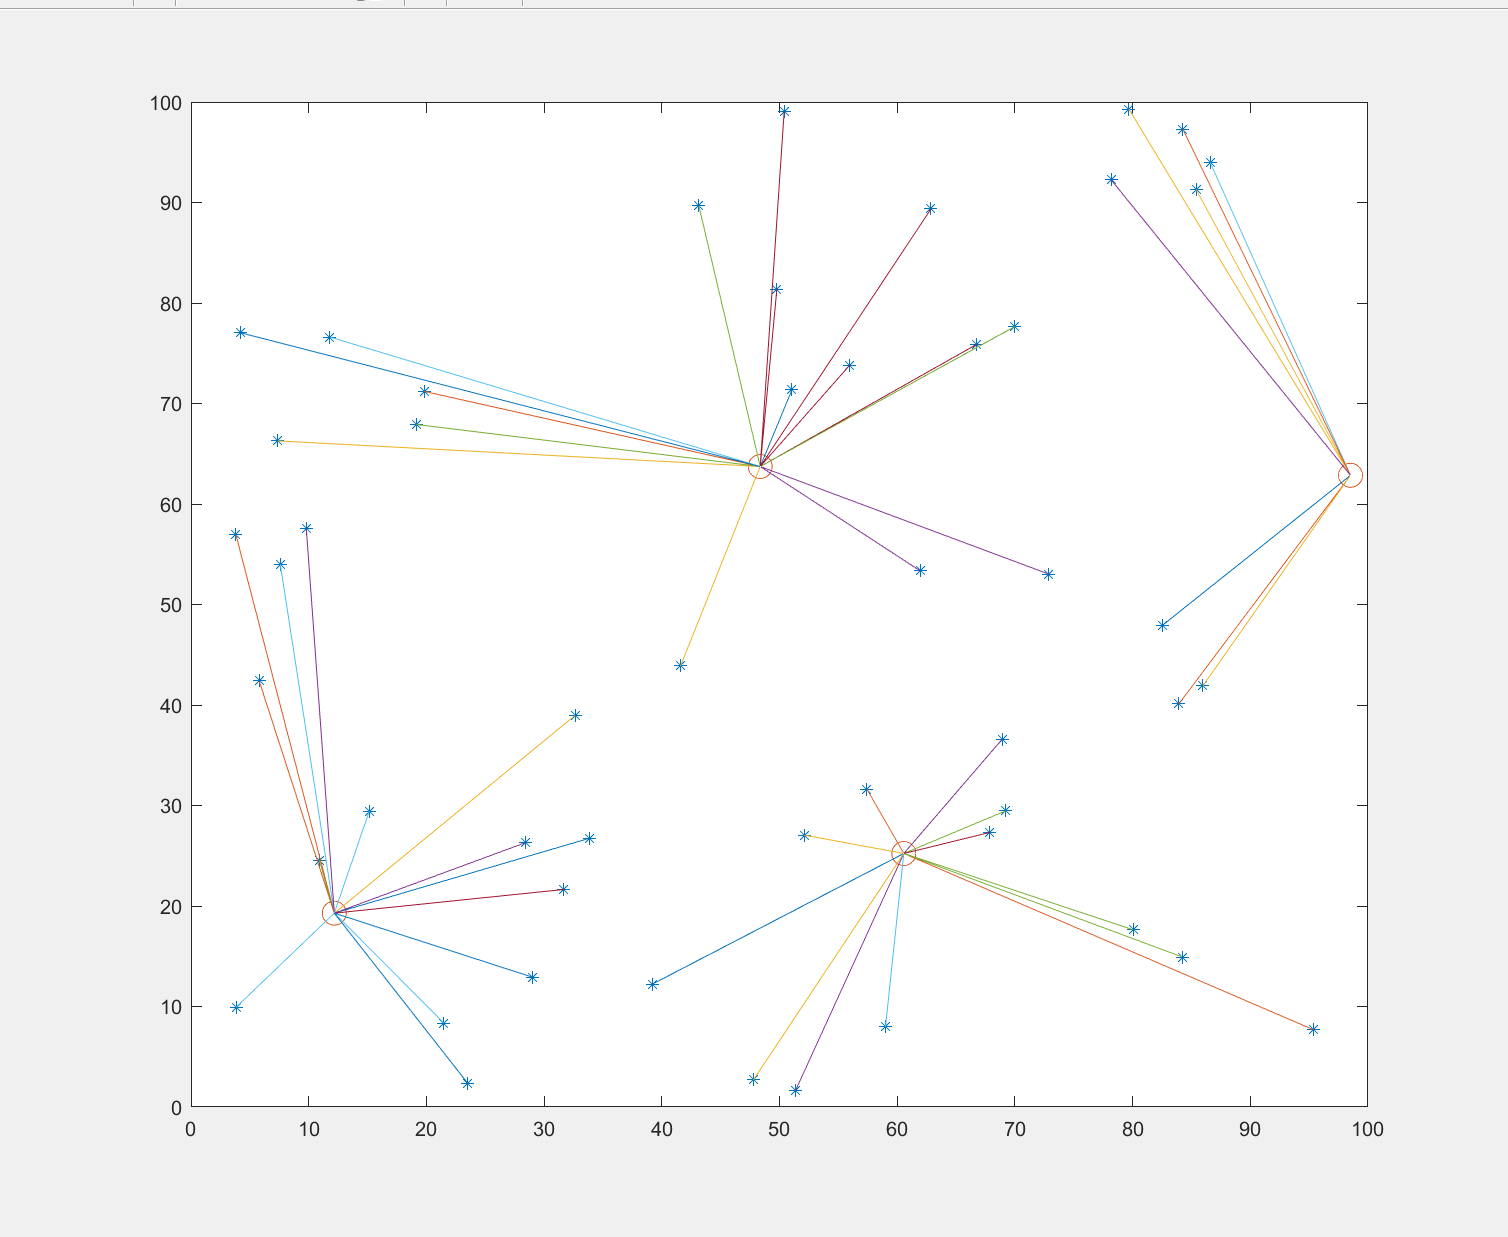
\includegraphics[scale=0.4]{distribution}
	\caption{An example with 50 users and 4 cells.}
	\label{fig:t}
\end{figure}

The pathloss of each user is given by
\begin{equation}
L_{uk} = d_{uk}^3
\end{equation}
where $d_{uk}$ is the distance from $u$-th user to $k$-th center.

The SIR $\gamma_1$ of 1st user in 1st cell, \textit{i.e.} $k_1=1$ can be represented as
\begin{align}\label{gamma}
	\gamma_1 &= \frac{P_1/L_{11}}{\sum_{u\neq 1}^{N}P_{u}/L_{u1}} \nonumber\\
	&= \frac{P_1/L_{11}}{\sum_{u=1}^{N}P_{u}/L_{u1} - P_1/L_{11}} \nonumber\\
	&= \frac{P_1}{L_{11}\sum_{u=1}^{N}P_{u}/L_{u1} - P_1}. 
\end{align}

From Eq. \eqref{gamma}, we have
\begin{align}
\frac{\gamma+1}{\gamma}P_1 &= L_{11}\sum_{u=1}^{N}P_{u}/L_{u1} \nonumber\\
& = L_{11} 
[1/L_{11}, 1/L_{21},\cdots, 1/L_{N1}]
\begin{bmatrix}
P_{1}\\
\cdots \\
P_{N}
\end{bmatrix}\nonumber\\
&=[1, L_{11}/L_{21},\cdots, L_{11}/L_{N1}]
\begin{bmatrix}
P_{1}\\
\cdots \\
P_{N}
\end{bmatrix}
\end{align}

By applying the balanced SIR algorithm on all users, the problem is formulated as
\begin{align}
\frac{\gamma+1}{\gamma}\bm{p} &= \bm{G}\bm{p} \nonumber\\
\frac{1}{\gamma}\bm{p} &= (\bm{G}-\bm{I})\bm{p}
\end{align}
where 
\begin{align}
\bm{G} = 
\begin{bmatrix}
1& L_{1k_1}/L_{2k_1}&\cdots& L_{1k_1}/L_{Nk_1}\\
L_{2k_2}/L_{1k_2}& 1&\cdots& L_{2k_2}/L_{Nk_2}\\
\vdots&\vdots&\vdots&\vdots\\
L_{Nk_N}/L_{1k_N}& L_{Nk_N}/L_{2k_N}&\cdots& 1
\end{bmatrix}
\quad
\bm{p} =
\begin{bmatrix}
P_{1}\\
P_{2}\\
\vdots\\
P_N
\end{bmatrix}
\end{align}
where the $k_u,u\in (1, N)$ means that the $u$-th user is distributed to $k$-th cell.

\textbf{Based on the \textit{Perron–Frobenius theorem}, there exists an eigenvector that all the elements are positive. Since $trace(G-I)=0$, there must exist an eigenvalue lager than 0.}

\section{Proof for $\bm{G}^U = (\bm{G}^D)^T$}
% For 1st user in 1st cell, \textit{i.e.} $k_1=1$
%\begin{align}\label{gammaD}
%\gamma_1 &= \frac{P_1/L_{11}}{\sum_{u\neq 1}^{N}P_{u}/L_{1k_u}} \nonumber\\
%&=\frac{P_1/L_{11}}{\sum_{u=1}^{N}P_{u}/L_{1k_u} - P_1/L_{11}} \nonumber\\
%&= \frac{P_1}{L_{11}\sum_{u=1}^{N}P_{u}/L_{1k_u} - P_1} 
%\end{align}
%The SIR for downlink is represented as
%\begin{align}
%\frac{\gamma+1}{\gamma}\bm{p}^D &= \bm{G}^D\bm{p}^D\\
%\frac{1}{\gamma}\bm{p}^D &= (\bm{G}^D-\bm{I})\bm{p}^D
%\end{align}
%where 
%\begin{align}
%\bm{G}^D = 
%\begin{bmatrix}
%1& L_{1k_1}/L_{1k_2}&\cdots& L_{1k_1}/L_{1k_N}\\
%L_{2k_2}/L_{2k_1}& 1&\cdots& L_{2k_2}/L_{2k_N}\\
%\vdots&\vdots&\vdots&\vdots\\
%L_{Nk_N}/L_{Nk_1}& L_{Nk_N}/L_{Nk_2}&\cdots& 1
%\end{bmatrix}
%\quad
%\bm{p}^D =
%\begin{bmatrix}
%P_{1}\\
%P_{2}\\
%\vdots\\
%P_N
%\end{bmatrix}
%\end{align}

\subsection{In BS-to-BS Matrix}
We assume N base stations, and a common channel. Let $L_i$ denote the user number of cell i. We define a geometry as show in Fig. \ref{fig:geomatrix}, where $g_{ikj}$ denotes the gain for user k in cell i to base station in cell j.% Let $p_i^U$ denote the received power by the BS of the i-th cell from any one users in this cell, so that the power vector is \begin{equation*}
%\bm P^U = \left[ \begin{matrix}
%p_1^U,p_2^U,\cdots,p_N^U
%\end{matrix}\right]^T 
%\end{equation*}
% The signal to interference ration can be expressed as:
%
%\begin{equation}
%\gamma_i^U = \frac{p_i^U}{\sum_{j=1}^N p_j^U \sum_{k=1}^{L_j} \frac{ g_{jki} }{g__{jkj}}}-p_i^u}
%\end{equation}


\begin{figure*}[th]
	\centering
	\includegraphics[width=0.7\linewidth]{"proof for the transpose/geomatrix"}
	\caption{Interference Geometry}
	\label{fig:geomatrix}
\end{figure*}

\subsubsection{SIR in Uplink}

Let $p_i^U$ denote the received power by the BS of the i-th cell from any one users in this cell, so that the power vector is \begin{equation*}
\bm P^U = \left[ \begin{matrix}
p_1^U,p_2^U,\cdots,p_N^U
\end{matrix}\right]^T. 
\end{equation*}
The signal to interference ration can be expressed as:

\begin{equation}
\gamma_i^U = \frac {p_i^U} { \sum\limits_{j=1}^N p_j^U \sum\limits_{k=1}^{L_j}\frac{ g_{jki} } { g__{jkj }} } - p_i^u }. \end{equation}

Thus, \begin{equation*}
G^U=[G_{ij}^U];
\end{equation*}
where \begin{equation}
G_{ij}^U = \sum^{L_j}_{k=1} \frac{g_{jki}}{g_{jkj}}.
\end{equation}

\subsubsection{SIR in Downlink}

Then we assumed $p_{ik}^D$ as the transmit power at BS of cell i to the k-th user in the same cell. So that the desired signal of which user received is \begin{equation*}
p_{desired}= p_{ik}^D \times g_{iki}.
\end{equation*}

And $Q_i$ represents the total transmit power for the i-th BS. Thus, we can get that
\begin{equation}
Q_i= \sum_{k=1}^{L_i} p_{ik}^D.
\end{equation}
so that the power vector in the downlink is \begin{equation*}
\bm Q = \left[ \begin{matrix}
Q_1,Q_2,\cdots,Q_N
\end{matrix}\right]^T. 
\end{equation*}

The SIR at the user k in cell i can be expressed as:
\begin{equation}
\gamma_{ik}^D = \frac{p_{desired} }{\sum\limits_{j=1}^N Q_jg_{ikj}-p_{desired}} = \frac{p_{ik}^D g_{iki}}{\sum\limits_{j=1}^N Q_jg_{ikj}-p_{ik}^D g_{iki}}
\end{equation}
By the global power control algorithm, we should set  $\gamma_i^D$ = $\gamma_{ik}^D$ (i=1,2,\dots,N). Generally, the SIR values are different form cell to cell, and within a given cell, the SIR will be different between uplink and downlink. Also by the global PCA, we need to balance the values of SIR in the downlink for each cell. Setting all $\gamma_i^D$to be equal leads to an eigenvalue equation problems, which is same like uplink. Hence,



\begin{align*}
\gamma_i^D&=\frac{\sum p_{desired} }{\sum\limits_{j=1}^N Q_j \sum\limits_{k=1}^{L_i} g_{ikj}-\sum p_{desired}}\\   
&=\frac{\sum p_{ik}^D g_{iki} } {\sum\limits_{j=1}^N Q_j \sum\limits_{k=1}^{L_i} g_{ikj}-\sum p_{ik}^D g_{iki}}\\
&=\frac{\sum p_{ik}^D  } {\sum\limits_{j=1}^N Q_j \sum\limits_{k=1}^{L_i} \frac{g_{ikj}}{g_{iki}}-\sum p_{ik}^D}
\end{align*}
By (3) we can get the SIR values of downlink is \begin{equation}
\gamma_i^D=\frac{Q_i  } {\sum\limits_{j=1}^N Q_j \sum\limits_{k=1}^{L_i} \frac{g_{ikj}}{g_{iki}}-Q_i}
\end{equation}

Thus,  \begin{equation*}
G^D=[G_{ij}^D];
\end{equation*}
where \begin{equation}
G_{ij}^D = \sum^{L_i}_{k=1} \frac{g_{ikj}}{g_{iki}}.
\end{equation}

\subsubsection{result}

Now, we list the matrix of uplink and downlink,
\begin{equation} \label{GU}
\bm G^U = \left[ \begin{matrix}
\sum\limits_{k=1}^{L_1}\frac{g_{1k1}}{g_{1k1}}&\sum\limits_{k=1}^{L_2}\frac{g_{2k1}}{g_{2k2}}&\cdots&\sum\limits_{k=1}^{L_N}\frac{g_{Nk1}}{g_{NkN}}\\
\sum\limits_{k=1}^{L_1}\frac{g_{1k2}}{g_{1k1}}&\sum\limits_{k=1}^{L_2}\frac{g_{2k2}}{g_{2k2}}&\cdots&\sum\limits_{k=1}^{L_N}\frac{g_{Nk2}}{g_{NkN}}\\
\vdots&\vdots&\ddots&\vdots\\
\sum\limits_{k=1}^{L_1}\frac{g_{1kN}}{g_{1k1}}&\sum\limits_{k=1}^{L_2}\frac{g_{2kN}}{g_{2k2}}&\cdots&\sum\limits_{k=1}^{L_N}\frac{g_{NkN}}{g_{NkN}}
\end{matrix}\right]. 
\end{equation}
\begin{equation} \label{GD}
\bm G^D = \left[ \begin{matrix}
\sum\limits_{k=1}^{L_1}\frac{g_{1k1}}{g_{1k1}}&\sum\limits_{k=1}^{L_1}\frac{g_{1k2}}{g_{1k1}}&\cdots&\sum\limits_{k=1}^{L_1}\frac{g_{1kN}}{g_{1k1}}\\
\sum\limits_{k=1}^{L_2}\frac{g_{2k1}}{g_{2k2}}&\sum\limits_{k=1}^{L_2}\frac{g_{2k2}}{g_{2k2}}&\cdots&\sum\limits_{k=1}^{L_2}\frac{g_{2kN}}{g_{2k2}}\\
\vdots&\vdots&\ddots&\vdots\\
\sum\limits_{k=1}^{L_N}\frac{g_{Nk1}}{g_{NkN}}&\sum\limits_{k=1}^{L_N}\frac{g_{Nk2}}{g_{Nk2}}&\cdots&\sum\limits_{k=1}^{L_N}\frac{g_{NkN}}{g_{NkN}}
\end{matrix}\right]. 
\end{equation}
The equations (\ref{GU}) and equation (\ref{GD}) reveals that 
\begin{equation*}
G^U\quad=\quad\left[G^D\right]^T.
\end{equation*}
The equation is only proved for the cell-to-cell matrix. Refer to the user-to-user matrix, we generate the matrix while recognize which cell the users belonging to. So it's unique, of which roles and columns have different definitions. That means we cannot discover an uplink gain matrix, which is the transpose of the downlink gain matrix.
%\bibliography{PCAref}
%\bibliographystyle{IEEEtran}
\end{document}


